\section{Recurrences}

To determine the complexity a recurrent algorithm, we need to solve the equation:
\[T(n)=2T\left(\frac{n}{2}\right)+c\cdot n\]
To solve this recurrence we may use three different tecniques: 
\begin{enumerate}
    \item Recursion tree.
    \item Substitution method.
    \item Masther method. 
\end{enumerate}

\subsection{Recursion tree}
In the recursion tree we expand nodes until we reach the base case. 
\begin{figure}[H]
    \centering
    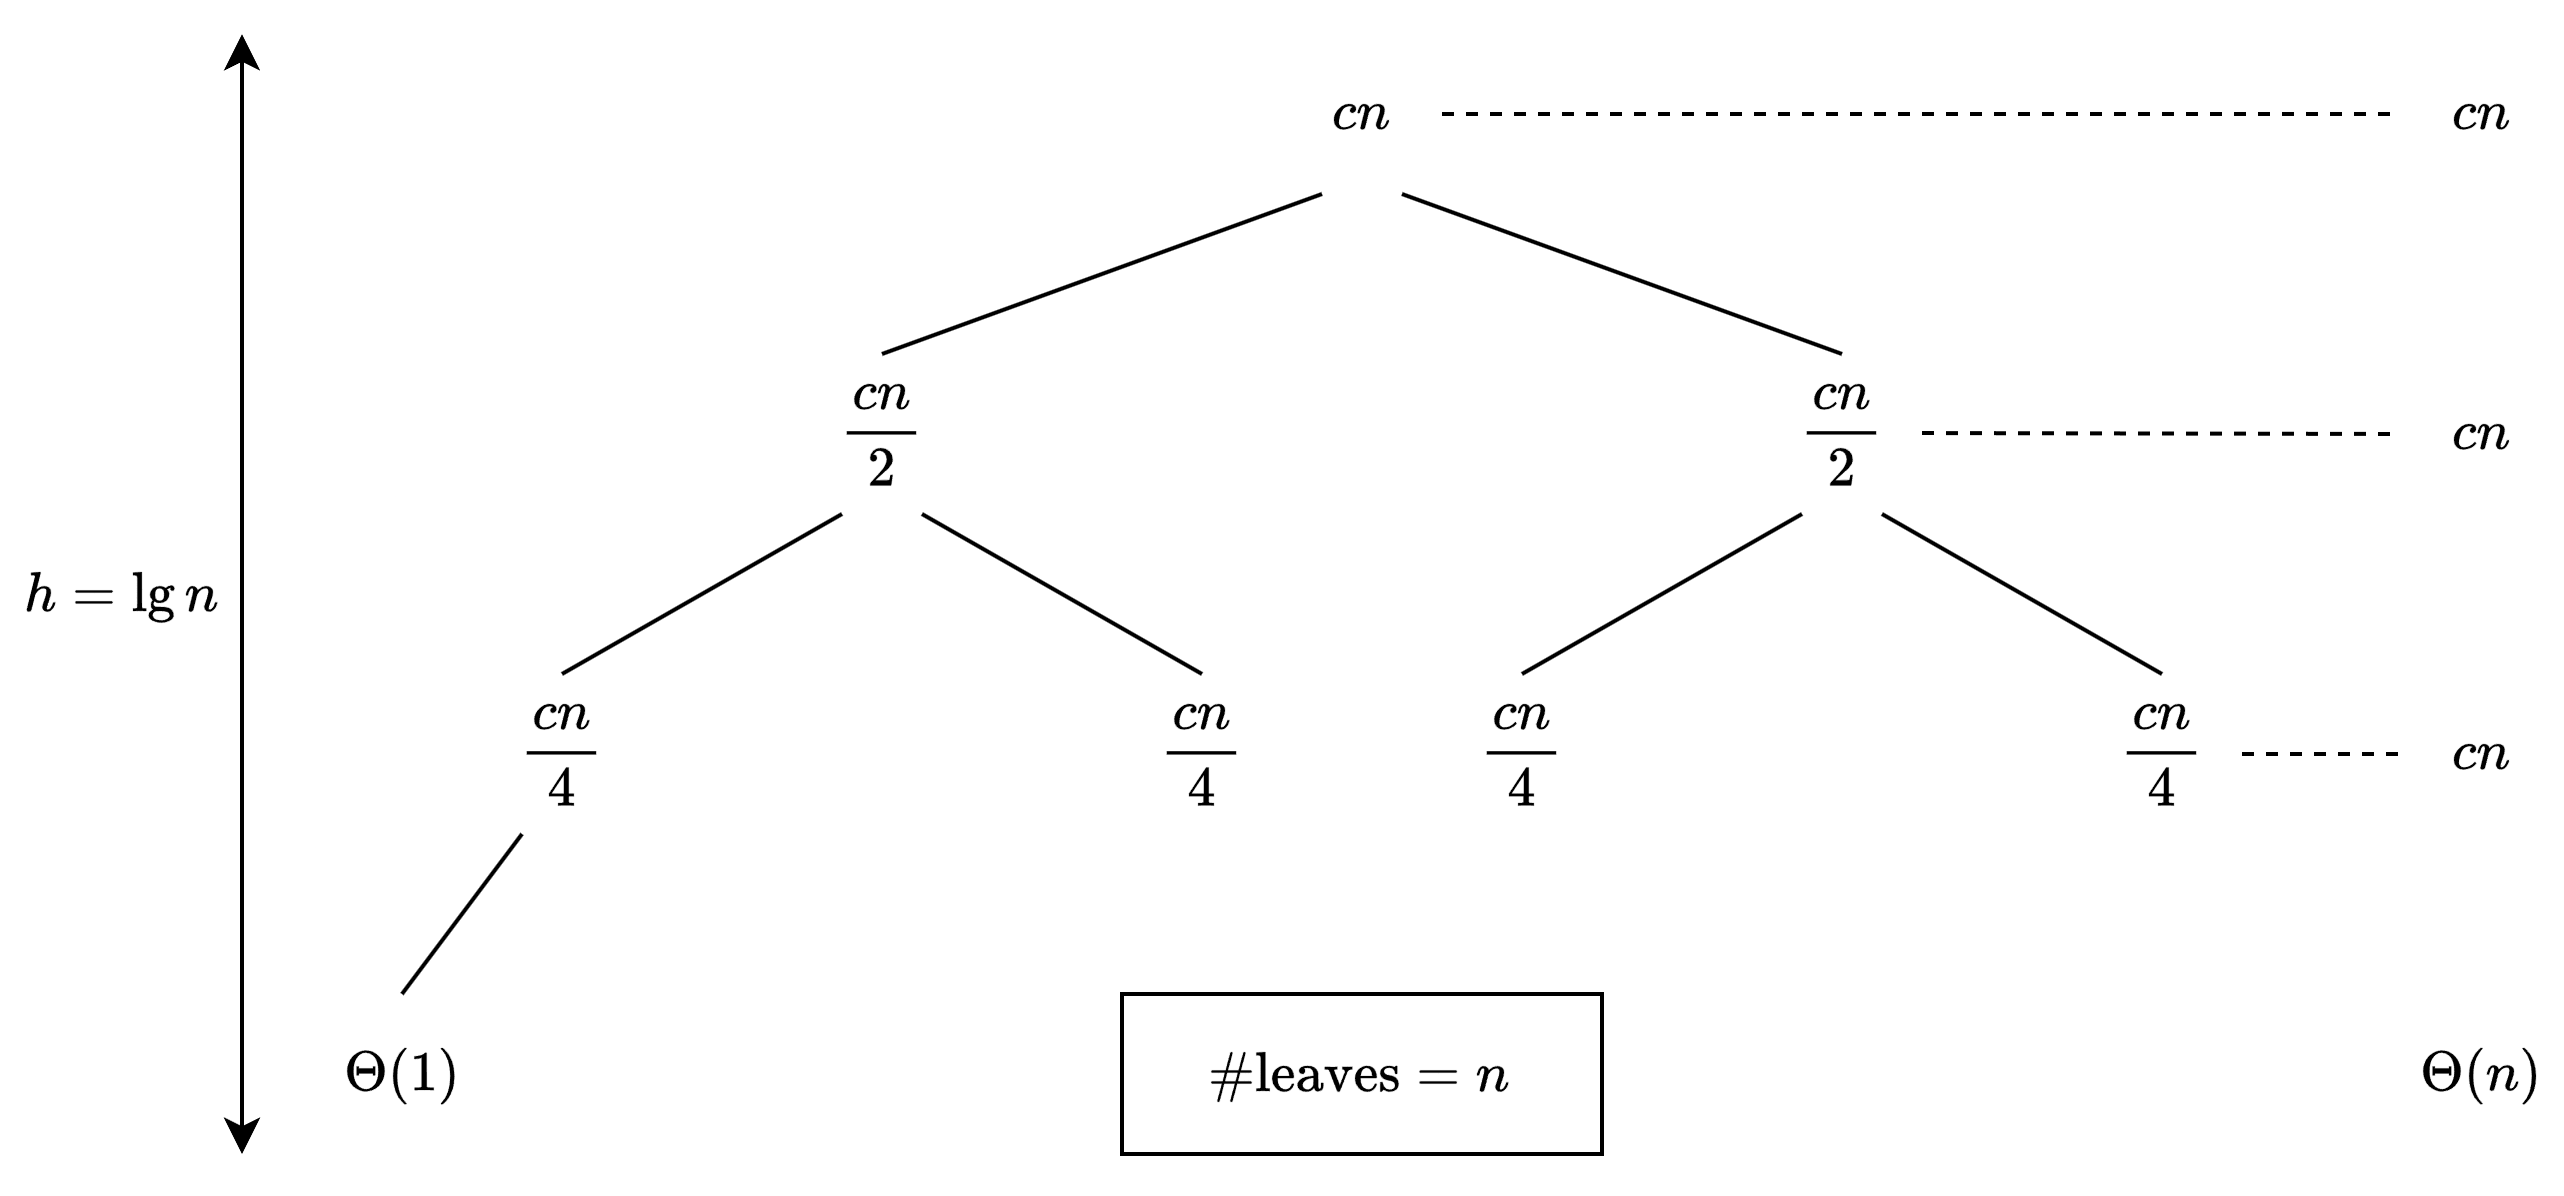
\includegraphics[width=0.75\linewidth]{images/tree.png}
    \caption{Partial recursion tree for merge sort algorithm}
\end{figure}
The depth of the tree is $h=\log_2n$, and the total number of leaves is $n$. 
Thus, the complexity can be computed as:
\[T(n)=\Theta(n\log_2n)\]
The merge sort outperforms insertion sort in the worst case, but in practice merge sort generally surpasses insertion sort for $n > 30$.

\subsection{Substitution method}
The substitution method is a general technique for solving recursive complexity equations. 
The steps are as follows:
\begin{enumerate}
    \item Guess the form of the solution based on preliminary analysis of the algorithm.
    \item Verify the guess by induction.
    \item Solve for any constants involved.
\end{enumerate}
\begin{example}
    Consider the expression:
    \[T(n)=4T\left(\frac{n}{2}\right)+n\]
    Assuming the base case $T(1)=\Theta(1)$, we can apply the substitution method:
    \begin{enumerate}
        \item Guess a solution of $\mathcal{O}(n^3)$, so we assume $T(k)\leq c k^3$ for $k<n$. 
        \item Verify by induction that $T(n)\leq c n^3$. 
    \end{enumerate}
\end{example}
This approach, while effective, may not always be straightforward.

\subsection{Master method}
To simplify the analysis, we can use the master method, applicable to recurrences of the form:
\[T(n)=aT\left(\frac{n}{b}\right)+f(n)\]
Here, $a\geq 1$, $b>1$, and $f(n)$ is asymptotically positive. 
While less general than the substitution method, it is more straightforward.

To apply the master method, compare $f(n)$ with $n^{\log_ba}$. 
There are three possible outcomes:
\begin{enumerate}
    \item If $f(n)=O(n^{\log_ba-\varepsilon})$ for some constant $\varepsilon > 0$, then
        \[T(n)=\Theta(n^{\log_ba})\]
    \item If $f(n)=\Theta(n^{\log_ba}\log^kn)$ for some constant $k \geq 0$, then: 
        \[T(n)=\Theta(n^{\log_ba}\log^{k+1}n)\]
    \item If $f(n)=\Omega(n^{\log_ba+\varepsilon})$ for some constant $\varepsilon > 0$ and $f(n)$ satisfies the regularity condition $a \cdot f\left(\frac{n}{b}\right) \leq c \cdot f(n)$ for some constant $c < 1$, then:
        \[T(n)=\Theta(f(n))\]
\end{enumerate}
\begin{example}
    Let's analyze the expression:
    \[T(n)=4T\left(\frac{n}{2}\right)+n\]
    In this case, we have $a=4$ and $b=2$, which gives us:
    \[n^{\log_ba}=n^2 \qquad f(n)=n\]
    Here, we find ourselves in the first case of the master theorem, where $f(n)=\mathcal{O}(n^{2-\varepsilon})$ for $\varepsilon=1$. 
    Thus, the solution is:
    \[T(n)=\Theta(n^2)\]

    Now consider the expression:
    \[T(n)=4T\left(\frac{n}{2}\right)+n^2\]
    Again, we have $a=4$ and $b=2$, leading to:
    \[n^{\log_ba}=n^2 \qquad f(n)=n^2\]
    In this scenario, we are in the second case of the theorem, where $f(n)=\Theta(n^2\log^kn)$ for $k=0$. 
    Therefore, the solution is:
    \[T(n)=\Theta(n^2\log n)\]

    Next, consider:
    \[T(n)=4T\left(\frac{n}{2}\right)+n^3\]
    With $a=4$ and $b=2$, we find:
    \[n^{\log_ba}=n^2 \qquad f(n)=n^3\]
    Here, we fall into the third case of the theorem, where $f(n)=\Omega(n^{2+\varepsilon})$ for $\varepsilon=1$. 
    Thus, the solution is:
    \[T(n)=\Theta(n^3)\]

    Finally, consider the expression:
    \[T(n)=4T\left(\frac{n}{2}\right)+\frac{n^2}{\log n}\]
    Again, we have $a=4$ and $b=2$ yielding:
    \[n^{\log_ba}=n^2 \qquad f(n)=\frac{n^2}{\log n}\]
    In this case, the master method does not apply. 
    Specifically, for any constant $\varepsilon > 0$, we have $n^\varepsilon = \omega(\log n)$, indicating that the conditions for the theorem are not satisfied.
\end{example}